% =====================================================================
%  Methods and Results (Tasks 1 and 4: case duration, disposal nature)
%  Needs: booktabs, float, graphicx, amsmath, caption (all in main.tex)
%  Figures: fig_segment_weights.pdf, fig_mixing_weights.pdf,
%           forgetting_curves.png (from the Kaggle notebook output)
%  Bibliography: add references_additions.bib to references.bib
% =====================================================================

\section{Methodology}
\label{sec:method}

\subsection{Problem setting}
Each of the five High Courts (Bombay, Delhi, Karnataka, Kerala, Madhya Pradesh) is one federated client that keeps its judgments locally. From the text of a judgment, with its operative ending removed, the model predicts three labels: the \emph{case duration} in days (Task~1, regressed as $y=\log(1+\text{days})$), the \emph{case type} (one of ten families, used as an auxiliary task and as input to Task~4), and the \emph{disposal nature} (Task~4: allowed, dismissed, disposed of, withdrawn; taken from the text-derived outcome label, since the metadata label is missing for every Delhi case). We use the 12{,}500 labelled judgments (2{,}500 per court, about 1{,}750 training cases per court) with the existing temporal 70/15/15 split within each court.

\paragraph{Leakage control.} All cases in the dataset were decided in 2024, so dates, years and case numbers in the text almost reveal the duration. We mask all dates, four-digit years and multi-digit numbers. Outcome words (\emph{allowed}, \emph{dismissed}, \emph{disposed of}, \emph{withdrawn}, \dots) are also masked so the disposal label cannot be copied from the text.

\subsection{Base model}
The encoder is InLegalBERT~\cite{paul2023inlegalbert} (RoBERTa-base~\cite{liu2019roberta} as a general-domain comparison), adapted with LoRA~\cite{hu2022lora} (rank 8 on the query and value projections); the encoder's own weights stay frozen. A case is represented by the mean of its token embeddings. Three heads follow: an MLP for duration (Huber loss on $y$), a linear case-type classifier, and an MLP for disposal nature that receives the case-type probabilities as extra input (the case type $\rightarrow$ disposal cascade of the proposal). The training loss is
\begin{equation}
\mathcal{L} = \mathcal{L}_{\text{Huber}}(\hat y, y) + 0.5\,\mathcal{L}_{\text{CE}}(\text{type}) + \mathcal{L}_{\text{CE}}^{w}(\text{disposal}),
\end{equation}
where the disposal classes are weighted by each court's own class frequencies. Only the trainable parameters (LoRA adapters and heads, about 1\% of the model) are exchanged with the server.

\paragraph{Federated training.} FedAvg~\cite{mcmahan2017communication} averages the clients' parameters weighted by their training set size; each round every court trains for one local epoch. Training runs for at most 30 rounds with early stopping after 4 rounds without improvement, and the model from the round with the lowest size-weighted validation loss is kept. All hyper-parameters (encoder, learning rate, truncation) are chosen on validation loss; test results are only reported.

\paragraph{Baselines.} \emph{Local only} (each court trains alone) and \emph{centralized} (all training data pooled, not private) bracket the federated methods. We compare FedProx~\cite{li2020federated}, FedAvgM~\cite{hsu2019fedavgm}, FedAdam~\cite{reddi2021adaptive}, loss-based client weighting $w_k \propto n_k e^{-\beta L_k}$ (in the spirit of FedLBW~\cite{fedlbw2026} for $\beta>0$ and q-FFL~\cite{li2020qffl} for $\beta<0$), FedAvg followed by one epoch of fine-tuning on each court (\emph{+ft}), and naive sequential training with EWC~\cite{kirkpatrick2017ewc}.

\subsection{Proposed method 1: task-specific reading of the judgment (TSR)}
Judgments are long, and a 256-token input forces a choice: the start holds the parties, the case type and the facts, while the end holds the reasoning that leads to the outcome. In preliminary runs, keeping only the start was better for duration and keeping the start and end was better for disposal (Table~\ref{tab:fl_ablation}). TSR removes this trade-off. The shared encoder embeds the first and the last 256 tokens of a judgment separately, giving $e_{\text{start}}$ and $e_{\text{end}}$. Each task $t$ has its own learned query $q_t$ and reads its own weighted combination:
\begin{equation}
w_{t,s} = \operatorname{softmax}_{s}\!\left(\frac{q_t^\top e_s}{\sqrt{H}}\right), \qquad
r_t = \sum_{s\in\{\text{start},\,\text{end}\}} w_{t,s}\, e_s ,
\end{equation}
where $H$ is the hidden size. The queries start at zero (equal weights) and are shared and averaged like the rest of the model. The learned weights $w_{t,\text{end}}$ show which part of a judgment each task relies on.

\subsection{Proposed method 2: per-task learned mixing of shared and local heads (PTM)}
The courts differ in different ways for different tasks: in Table~\ref{tab:decoupled}, keeping the case-type head local helps a lot, keeping the disposal head local helps disposal, and keeping the duration head local hurts. A fixed choice of which heads to share therefore cannot suit every task. In PTM, every court $k$ keeps, for each task $t$, both the shared head $g_t$ and its own copy $g_t^{(k)}$, and learns how much to trust each:
\begin{equation}
f_t^{(k)}(r_t) = a_{k,t}\, g_t(r_t) + \bigl(1-a_{k,t}\bigr)\, g_t^{(k)}(r_t), \qquad a_{k,t} = \sigma(\alpha_{k,t}).
\end{equation}
The shared heads are averaged by the server; the local heads and the mixing logits $\alpha_{k,t}$ (initialised at $0$, i.e.\ $a_{k,t}=0.5$) never leave the court. The learned $a_{k,t}$ give a per-court, per-task measure of how useful collaboration is. Blending global and local models per client has been proposed before (APFL~\cite{deng2020apfl}, FedALA~\cite{zhang2023fedala}); PTM applies the blend separately to each task of a multi-task model. The mixing logits and the TSR queries use a larger learning rate ($10^{-2}$) than the rest of the model so that they can move within the training budget.

\subsection{Federated continual onboarding}
In practice, courts join a federation over time. We simulate this by adding the courts one at a time; each new court trains the shared model for three epochs. Each court's task heads are kept local, so they cannot be overwritten by later courts; the shared encoder is protected with EWC~\cite{kirkpatrick2017ewc} restricted to the shared parameters, a replay buffer of 16 training cases from each earlier court mixed into later training~\cite{rolnick2019replay}, or both. After every new court, all courts that have already joined are re-evaluated, which lets us measure \emph{forgetting}: the change in a court's error between the moment it joined and the end.

\subsection{Evaluation}
For duration we report the mean absolute error of $\log(1+\text{days})$ (MAE$_{\log}$), Spearman's rank correlation, and the macro-F1 over four duration buckets ($\le$30, 31--180, 181--730 and $>$730 days). For disposal nature and case type we report macro-F1. Metrics are computed per court on the test set and averaged; because the project targets heterogeneity, we also report the \emph{worst court} for duration and disposal. The main comparisons use three seeds (mean $\pm$ standard deviation).

% =====================================================================
\section{Results}
\label{sec:results}

\subsection{Encoder and input selection}
Table~\ref{tab:fl_ablation} shows the FedAvg runs used to fix the setting. InLegalBERT is better than RoBERTa, and a learning rate of $5{\times}10^{-4}$ is better than $2{\times}10^{-4}$. The two truncations trade off against each other: the first 256 tokens give the lowest duration error, while the first and last 128 tokens give much better disposal F1 (0.542 against 0.486) and the lower combined validation loss. This trade-off motivated TSR.

\begin{table}[H]
\centering
\footnotesize
\setlength{\tabcolsep}{4pt}
\begin{tabular}{l c l c ccc c cc}
\toprule
& & & & \multicolumn{3}{c}{\textbf{Duration}} & \textbf{Disposal} & \multicolumn{2}{c}{\textbf{Worst court}} \\
\cmidrule(lr){5-7}\cmidrule(lr){8-8}\cmidrule(lr){9-10}
\textbf{Encoder} & \textbf{LR} & \textbf{Tokens} & Val.\ loss$\downarrow$ & MAE$_{\log}\downarrow$ & Spearman$\uparrow$ & F1$_4\uparrow$ & F1$\uparrow$ & MAE$_{\log}\downarrow$ & Disp.\ F1$\uparrow$ \\
\midrule
InLegalBERT & $2{\times}10^{-4}$ & first 256 & 2.260 & 1.449 & 0.610 & 0.427 & 0.481 & 1.720 & 0.361 \\
InLegalBERT & $5{\times}10^{-4}$ & first 256 & 2.226 & 1.431 & 0.611 & 0.443 & 0.486 & 1.759 & 0.402 \\
InLegalBERT & $5{\times}10^{-4}$ & first+last 128$^\dagger$ & 2.164 & 1.460 & 0.599 & 0.434 & 0.542 & 1.886 & 0.447 \\
\midrule
RoBERTa-base & $2{\times}10^{-4}$ & first 256 & 2.419 & 1.505 & 0.590 & 0.406 & 0.462 & 1.802 & 0.354 \\
RoBERTa-base & $5{\times}10^{-4}$ & first 256 & 2.238 & 1.436 & 0.591 & 0.432 & 0.471 & 1.703 & 0.388 \\
RoBERTa-base & $5{\times}10^{-4}$ & first+last 128$^\dagger$ & 2.173 & 1.553 & 0.549 & 0.397 & 0.547 & 1.968 & 0.457 \\
\bottomrule
\end{tabular}
\caption{Setting selection with FedAvg (seed 0). $^\dagger$Chosen on validation loss.}
\label{tab:fl_ablation}
\end{table}

\subsection{Federated baselines}
Table~\ref{tab:fl_results} compares the federated algorithms with local and centralized training. On average duration, local training, centralized training and FedAvg with fine-tuning are tied (MAE$_{\log}$ 1.462), and plain FedAvg is slightly behind (1.474). Pooling all the data does not beat training each court alone, a sign of how different the courts are. Fine-tuning the federated model on each court is the most useful addition: compared with FedAvg it lowers the worst court's duration error from 1.888 to 1.789 (about five standard deviations) and raises disposal F1 from 0.542 to 0.554. None of FedProx, FedAvgM, FedAdam or loss-based weighting improves clearly on FedAvg. Giving more weight to courts that already fit well ($\beta=+1$) badly hurts the worst court (2.175), confirming the fairness concern that motivated this project, and naive sequential training is the weakest method.

\begin{table}[H]
\centering
\footnotesize
\setlength{\tabcolsep}{3.5pt}
\renewcommand{\arraystretch}{1.08}
\begin{tabular}{l c ccc c cc}
\toprule
& & \multicolumn{3}{c}{\textbf{Task 1: duration}} & \textbf{Task 4} & \multicolumn{2}{c}{\textbf{Worst court}} \\
\cmidrule(lr){3-5}\cmidrule(lr){6-6}\cmidrule(lr){7-8}
\textbf{Method} & Val.\ loss$\downarrow$ & MAE$_{\log}\downarrow$ & Spearman$\uparrow$ & F1$_4\uparrow$ & Disp.\ F1$\uparrow$ & MAE$_{\log}\downarrow$ & Disp.\ F1$\uparrow$ \\
\midrule
\multicolumn{8}{l}{\textit{Mean $\pm$ std over 3 seeds}} \\
Local only & \textbf{2.031}\,{\scriptsize$\pm$0.037} & \textbf{1.462}\,{\scriptsize$\pm$0.025} & 0.579\,{\scriptsize$\pm$0.009} & 0.427\,{\scriptsize$\pm$0.012} & 0.551\,{\scriptsize$\pm$0.013} & 1.825\,{\scriptsize$\pm$0.068} & \textbf{0.478}\,{\scriptsize$\pm$0.020} \\
Centralized & 2.046\,{\scriptsize$\pm$0.055} & \textbf{1.462}\,{\scriptsize$\pm$0.021} & 0.589\,{\scriptsize$\pm$0.009} & 0.430\,{\scriptsize$\pm$0.010} & \textbf{0.561}\,{\scriptsize$\pm$0.008} & 1.852\,{\scriptsize$\pm$0.015} & 0.457\,{\scriptsize$\pm$0.002} \\
FedAvg & 2.166\,{\scriptsize$\pm$0.002} & 1.474\,{\scriptsize$\pm$0.023} & 0.595\,{\scriptsize$\pm$0.013} & 0.427\,{\scriptsize$\pm$0.007} & 0.542\,{\scriptsize$\pm$0.001} & 1.888\,{\scriptsize$\pm$0.009} & 0.449\,{\scriptsize$\pm$0.008} \\
FedAvg + fine-tuning & 2.101\,{\scriptsize$\pm$0.007} & \textbf{1.462}\,{\scriptsize$\pm$0.035} & 0.595\,{\scriptsize$\pm$0.021} & \textbf{0.437}\,{\scriptsize$\pm$0.009} & 0.554\,{\scriptsize$\pm$0.007} & \textbf{1.789}\,{\scriptsize$\pm$0.020} & 0.462\,{\scriptsize$\pm$0.029} \\
\midrule
\multicolumn{8}{l}{\textit{Single seed (seed 0)}} \\
FedAvgM & 2.120 & 1.466 & 0.592 & 0.422 & 0.543 & 1.812 & 0.462 \\
FedProx ($\mu{=}0.01$) & 2.141 & 1.465 & \textbf{0.599} & 0.429 & 0.529 & 1.878 & 0.446 \\
FedProx ($\mu{=}0.1$) & 2.148 & 1.489 & 0.589 & 0.424 & 0.534 & 1.898 & 0.466 \\
FedAdam & 2.193 & 1.471 & 0.590 & 0.429 & 0.532 & 1.864 & 0.445 \\
Loss-weighting ($\beta{=}{-}1$) & 2.170 & \textbf{1.462} & 0.595 & 0.430 & 0.534 & 1.832 & 0.447 \\
Loss-weighting ($\beta{=}{+}1$) & 2.347 & 1.532 & 0.561 & 0.411 & 0.535 & 2.175 & 0.384 \\
Sequential EWC (naive) & 2.856 & 1.634 & 0.505 & 0.378 & 0.453 & 2.148 & 0.352 \\
\bottomrule
\end{tabular}
\caption{Federated baselines. InLegalBERT with LoRA, first and last 128 tokens, learning rate $5{\times}10^{-4}$; test set, mean over the five courts. Bold: best in each column.}
\label{tab:fl_results}
\end{table}

\subsection{Which heads should be shared?}
Table~\ref{tab:decoupled} keeps the shared encoder but holds some task heads local to each court, never averaged. Keeping the \emph{case-type} head local raises its F1 from 0.774 to 0.919: case-type families are recorded differently in each court. Keeping the \emph{disposal} head local gives the best disposal F1 (0.565) and the best worst-court disposal F1 (0.494). Keeping the \emph{duration} head local, by contrast, makes duration worse (1.494 against 1.474), and so does every other variant with local heads (1.481--1.531). No fixed choice is best for all tasks, which motivates learning the choice (PTM).

\begin{table}[H]
\centering
\footnotesize
\setlength{\tabcolsep}{4pt}
\renewcommand{\arraystretch}{1.08}
\begin{tabular}{l c cc c c cc}
\toprule
& & \multicolumn{2}{c}{\textbf{Duration}} & \textbf{Disposal} & \textbf{Case type} & \multicolumn{2}{c}{\textbf{Worst court}} \\
\cmidrule(lr){3-4}\cmidrule(lr){5-5}\cmidrule(lr){6-6}\cmidrule(lr){7-8}
\textbf{Heads kept local} & Val.\ loss$\downarrow$ & MAE$_{\log}\downarrow$ & Spearman$\uparrow$ & F1$\uparrow$ & F1$\uparrow$ & MAE$_{\log}\downarrow$ & Disp.\ F1$\uparrow$ \\
\midrule
None (FedAvg, 3 seeds) & 2.166 & \textbf{1.474} & \textbf{0.595} & 0.542 & 0.774 & 1.888 & 0.449 \\
Duration & 2.172 & 1.494 & 0.582 & 0.548 & 0.740 & 1.814 & 0.447 \\
Disposal nature & 2.267 & 1.531 & 0.568 & \textbf{0.565} & 0.684 & 1.995 & \textbf{0.494} \\
Case type + disposal & 2.186 & 1.531 & 0.572 & 0.562 & 0.918 & 1.968 & 0.484 \\
All three heads & \textbf{2.100} & 1.481 & 0.564 & 0.531 & \textbf{0.919} & \textbf{1.810} & 0.447 \\
\bottomrule
\end{tabular}
\caption{Fixed task-decoupled FedAvg: the encoder is always shared, the listed heads are kept per court. Same settings as Table~\ref{tab:fl_results}; decoupled variants are single runs (seed 0).}
\label{tab:decoupled}
\end{table}

\subsection{Proposed methods}
Table~\ref{tab:proposed} gives the main result. \textbf{Task-specific reading (TSR) is the largest improvement in the project.} With FedAvg it lowers the duration error from 1.474 to 1.347 (about six standard deviations), raises Spearman's correlation from 0.595 to 0.632, and lowers the worst court's duration error from 1.888 to 1.704. It also improves local and centralized training, so it is a better model rather than a federated effect. With TSR, federated training is better on duration than both local (1.390) and centralized (1.372) training with the same architecture, which plain FedAvg was not; the local and centralized TSR runs are single seeds, so this comparison is indicative.

TSR alone does not improve disposal (0.539), and it lowers case-type F1 compared with personalised variants. Adding personalisation fixes this. \textbf{PTM and fine-tuning are interchangeable routes to the same result}: TSR with PTM (1.370 / 0.554 / 0.913) and TSR with fine-tuning (1.367 / 0.560 / 0.913) are within noise of each other, but PTM personalises in a single training stage and its weights are interpretable. Combining both gives the best duration and correlation (1.347, 0.635) and the best case-type F1 (0.916), but by margins within one standard deviation; the combined validation loss does not separate the three personalised TSR variants (2.065--2.084). Without TSR, PTM behaves like keeping heads local: it improves case type (0.908) and the worst court's disposal (0.475) but worsens duration (1.506).

Compared with the best baseline (FedAvg with fine-tuning), TSR with PTM and fine-tuning reduces the duration error by 0.115 and the worst court's duration error by 0.080, while matching disposal F1 (0.557 against 0.554) and improving case-type F1 (0.916 against 0.900).

\begin{table}[H]
\centering
\footnotesize
\setlength{\tabcolsep}{3pt}
\renewcommand{\arraystretch}{1.08}
\begin{tabular}{l c cc c c cc}
\toprule
& & \multicolumn{2}{c}{\textbf{Duration}} & \textbf{Disposal} & \textbf{Case type} & \multicolumn{2}{c}{\textbf{Worst court}} \\
\cmidrule(lr){3-4}\cmidrule(lr){5-5}\cmidrule(lr){6-6}\cmidrule(lr){7-8}
\textbf{Method} & Val.\ loss$\downarrow$ & MAE$_{\log}\downarrow$ & Spearman$\uparrow$ & F1$\uparrow$ & F1$\uparrow$ & MAE$_{\log}\downarrow$ & Disp.\ F1$\uparrow$ \\
\midrule
\multicolumn{8}{l}{\textit{Baselines (single view, 3 seeds)}} \\
Local only & \textbf{2.031}\,{\scriptsize$\pm$0.037} & 1.462\,{\scriptsize$\pm$0.025} & 0.579\,{\scriptsize$\pm$0.009} & 0.551\,{\scriptsize$\pm$0.013} & 0.894\,{\scriptsize$\pm$0.019} & 1.825\,{\scriptsize$\pm$0.068} & \textbf{0.478}\,{\scriptsize$\pm$0.020} \\
Centralized & 2.046\,{\scriptsize$\pm$0.055} & 1.462\,{\scriptsize$\pm$0.021} & 0.589\,{\scriptsize$\pm$0.009} & \textbf{0.561}\,{\scriptsize$\pm$0.008} & 0.853\,{\scriptsize$\pm$0.028} & 1.852\,{\scriptsize$\pm$0.015} & 0.457\,{\scriptsize$\pm$0.002} \\
FedAvg & 2.166\,{\scriptsize$\pm$0.002} & 1.474\,{\scriptsize$\pm$0.023} & 0.595\,{\scriptsize$\pm$0.013} & 0.542\,{\scriptsize$\pm$0.001} & 0.774\,{\scriptsize$\pm$0.026} & 1.888\,{\scriptsize$\pm$0.009} & 0.449\,{\scriptsize$\pm$0.008} \\
FedAvg + ft & 2.101\,{\scriptsize$\pm$0.007} & 1.462\,{\scriptsize$\pm$0.035} & 0.595\,{\scriptsize$\pm$0.021} & 0.554\,{\scriptsize$\pm$0.007} & 0.900\,{\scriptsize$\pm$0.014} & 1.789\,{\scriptsize$\pm$0.020} & 0.462\,{\scriptsize$\pm$0.029} \\
\midrule
\multicolumn{8}{l}{\textit{Proposed (3 seeds)}} \\
PTM & 2.117\,{\scriptsize$\pm$0.013} & 1.506\,{\scriptsize$\pm$0.025} & 0.552\,{\scriptsize$\pm$0.012} & 0.549\,{\scriptsize$\pm$0.006} & 0.908\,{\scriptsize$\pm$0.017} & 1.855\,{\scriptsize$\pm$0.025} & 0.475\,{\scriptsize$\pm$0.009} \\
PTM + ft & 2.139\,{\scriptsize$\pm$0.056} & 1.488\,{\scriptsize$\pm$0.038} & 0.582\,{\scriptsize$\pm$0.016} & 0.555\,{\scriptsize$\pm$0.004} & 0.914\,{\scriptsize$\pm$0.004} & 1.845\,{\scriptsize$\pm$0.043} & \textbf{0.481}\,{\scriptsize$\pm$0.014} \\
TSR & 2.099\,{\scriptsize$\pm$0.019} & \textbf{1.347}\,{\scriptsize$\pm$0.013} & 0.632\,{\scriptsize$\pm$0.007} & 0.539\,{\scriptsize$\pm$0.012} & 0.844\,{\scriptsize$\pm$0.041} & \textbf{1.704}\,{\scriptsize$\pm$0.033} & 0.427\,{\scriptsize$\pm$0.026} \\
TSR + ft & \textbf{2.065}\,{\scriptsize$\pm$0.027} & 1.367\,{\scriptsize$\pm$0.011} & 0.630\,{\scriptsize$\pm$0.003} & \textbf{0.560}\,{\scriptsize$\pm$0.018} & 0.913\,{\scriptsize$\pm$0.003} & 1.716\,{\scriptsize$\pm$0.020} & 0.471\,{\scriptsize$\pm$0.022} \\
TSR + PTM & \textbf{2.065}\,{\scriptsize$\pm$0.017} & 1.370\,{\scriptsize$\pm$0.018} & 0.628\,{\scriptsize$\pm$0.005} & 0.554\,{\scriptsize$\pm$0.007} & 0.913\,{\scriptsize$\pm$0.008} & 1.716\,{\scriptsize$\pm$0.044} & 0.476\,{\scriptsize$\pm$0.012} \\
TSR + PTM + ft & 2.084\,{\scriptsize$\pm$0.022} & \textbf{1.347}\,{\scriptsize$\pm$0.019} & \textbf{0.635}\,{\scriptsize$\pm$0.005} & 0.557\,{\scriptsize$\pm$0.006} & \textbf{0.916}\,{\scriptsize$\pm$0.003} & 1.709\,{\scriptsize$\pm$0.036} & 0.473\,{\scriptsize$\pm$0.015} \\
\midrule
\multicolumn{8}{l}{\textit{TSR without federation (single seed)}} \\
Local only + TSR & 2.041 & 1.390 & 0.623 & 0.513 & 0.845 & 1.704 & 0.373 \\
Centralized + TSR & 2.020 & 1.372 & 0.628 & 0.554 & 0.897 & 1.711 & 0.423 \\
\bottomrule
\end{tabular}
\caption{Proposed methods. TSR: task-specific reading of the first and last 256 tokens; PTM: per-task learned mixing of shared and local heads; ft: one epoch of fine-tuning per court after federated training. Federated rows use FedAvg. Test set, mean over courts. Bold: best in each column among the 3-seed rows.}
\label{tab:proposed}
\end{table}

\subsection{What the model learned}
\paragraph{Where each task reads.} Figure~\ref{fig:segw} shows the learned attention on the end of the judgment. The pattern is the same in every court and under federated, local and centralized training: \emph{case type} reads mainly the start (13--25\% on the end), where the petition type and case number appear; \emph{disposal nature} reads mainly the end (65--86\%), where the reasoning leading to the outcome is; \emph{duration} uses both (49--72\%). This explains why duration gained most from TSR: with a single 256-token view it had to give up either the facts or the later reasoning. Federated training makes the disposal head lean further towards the end (76--86\%) than local or centralized training (65--83\%). The task-specific pattern indicates that TSR does more than add context; a single-view model with 512 tokens would be needed to quantify how much of the gain comes from the extra tokens alone.

\begin{figure}[H]
\centering
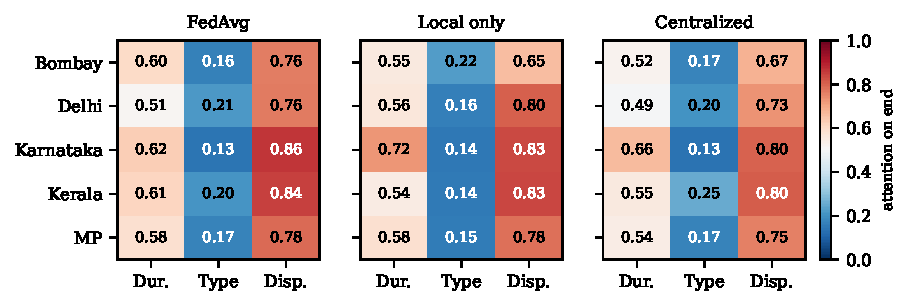
\includegraphics[width=0.92\linewidth]{fig_segment_weights.pdf}
\caption{TSR: share of attention on the end of the judgment, per court and task (0.5 = equal; red = end, blue = start). Mean over 3 seeds (FedAvg) or seed 0 (local, centralized).}
\label{fig:segw}
\end{figure}

\paragraph{How much each court trusts the shared heads.} Figure~\ref{fig:mixw} shows the learned weights $a_{k,t}$ on the shared head. In every court and with both architectures, duration relies most on the shared head (0.34--0.44), disposal less (0.16--0.24) and case type hardly at all (0.04--0.09). PTM thus recovers the ordering found by the fixed experiments in Table~\ref{tab:decoupled} on its own, per court, without trying every combination. The court differences for duration are consistent across seeds (standard deviation 0.01--0.03): Kerala relies most on the shared duration head (0.43--0.44) and Bombay least (0.34--0.36).

\begin{figure}[H]
\centering
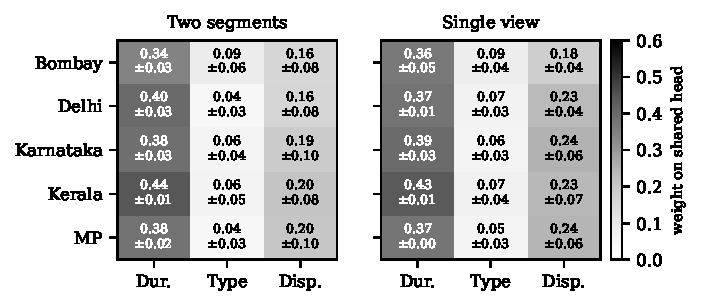
\includegraphics[width=0.66\linewidth]{fig_mixing_weights.pdf}
\caption{PTM: learned weight on the shared head per court and task (1 = shared only, 0 = own head only), mean $\pm$ std over 3 seeds.}
\label{fig:mixw}
\end{figure}

\subsection{Courts joining over time}
Table~\ref{tab:continual} and Figure~\ref{fig:forget} show federated continual onboarding. Replay roughly halves the forgetting of duration (0.089 to 0.043), while EWC alone does not affect it (0.097) but gives the lowest forgetting for disposal (0.017). The two are complementary: together they give the lowest duration forgetting (0.032) and low disposal forgetting (0.019). Forgetting is not one-way; several courts drop and then partly recover as later courts join (Figure~\ref{fig:forget}). Adding courts one at a time still costs accuracy: the best continual variant (1.547) is 0.07 worse than FedAvg training all courts together (1.474). The joining order does not change the average result, but it changes which court bears the cost: with Madhya Pradesh, the most distinct court, joining first, its own disposal F1 falls the most; with Madhya Pradesh last, disposal forgetting disappears ($-0.004$) and the duration forgetting concentrates on Kerala (+0.241), which joined just before the most different courts.

\begin{table}[H]
\centering
\footnotesize
\setlength{\tabcolsep}{3pt}
\renewcommand{\arraystretch}{1.08}
\begin{tabular}{l c c l cc c cc cc}
\toprule
& & & & \multicolumn{2}{c}{\textbf{Duration}} & \textbf{Disposal} & \multicolumn{2}{c}{\textbf{Worst court}} & \multicolumn{2}{c}{\textbf{Forgetting}$\downarrow$} \\
\cmidrule(lr){5-6}\cmidrule(lr){7-7}\cmidrule(lr){8-9}\cmidrule(lr){10-11}
\textbf{Strategy} & \textbf{EWC $\lambda$} & \textbf{Replay} & \textbf{Order} & MAE$_{\log}\downarrow$ & Spearman$\uparrow$ & F1$\uparrow$ & MAE$_{\log}\downarrow$ & Disp.\ F1$\uparrow$ & MAE$_{\log}$ & Disp.\ F1 \\
\midrule
Naive & -- & -- & MP first & 1.627 & 0.522 & 0.513 & 1.986 & 0.431 & 0.089 & 0.039 \\
EWC & 100 & -- & MP first & 1.635 & 0.513 & \textbf{0.524} & 2.005 & \textbf{0.468} & 0.097 & 0.017 \\
Replay & -- & 16 & MP first & \textbf{1.547} & 0.545 & 0.502 & 1.908 & 0.440 & 0.043 & 0.031 \\
EWC + replay & 100 & 16 & MP first & \textbf{1.547} & \textbf{0.560} & 0.511 & \textbf{1.876} & 0.453 & \textbf{0.032} & 0.019 \\
EWC + replay & 100 & 16 & MP last & 1.563 & 0.542 & \textbf{0.524} & 1.891 & 0.439 & 0.060 & \textbf{$-$0.004} \\
\midrule
\multicolumn{4}{l}{\textit{FedAvg, all courts at once (3 seeds)}} & 1.474 & 0.595 & 0.542 & 1.888 & 0.449 & -- & -- \\
\bottomrule
\end{tabular}
\caption{Federated continual onboarding, all task heads kept per court. ``MP first'': Madhya Pradesh, Bombay, Delhi, Kerala, Karnataka; ``MP last'': the reverse. Test set, single runs (seed 0), after the last court has joined. Forgetting: change between right after a court joined and the end (increase in MAE$_{\log}$, decrease in disposal F1), averaged over courts; negative values mean a court improved. A repeat of the replay configuration with only Delhi and Kerala swapped differed by 0.021 in MAE$_{\log}$ and 0.032 in duration forgetting, indicating the run-to-run variation.}
\label{tab:continual}
\end{table}

\begin{figure}[H]
\centering
\IfFileExists{forgetting_curves.png}{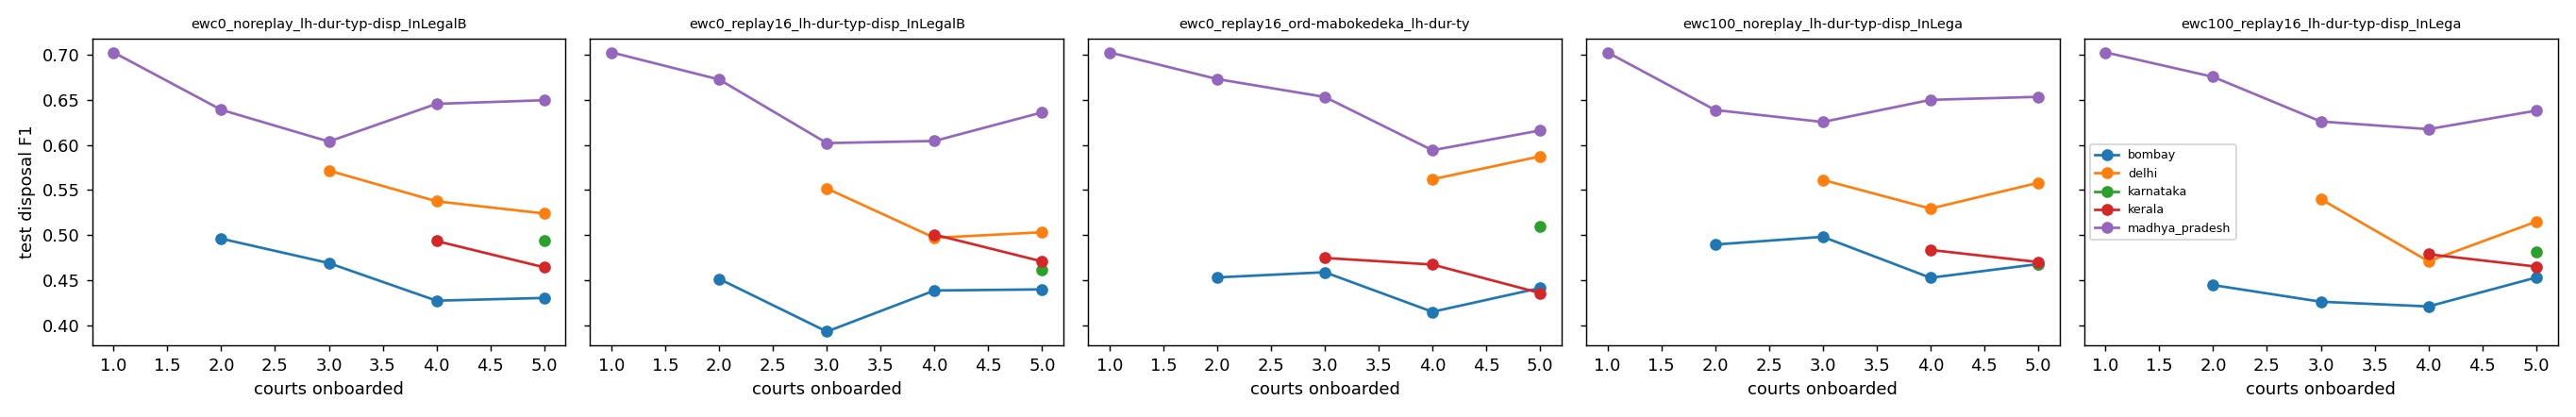
\includegraphics[width=\linewidth]{forgetting_curves.png}}{\fbox{\parbox{0.9\linewidth}{\centering Upload \texttt{forgetting\_curves.png} from the Kaggle notebook output.}}}
\caption{Test disposal F1 of each court as more courts join (one panel per strategy, Madhya Pradesh first).}
\label{fig:forget}
\end{figure}

\subsection{Limitations}
The local and centralized TSR results, the decoupled variants and the continual runs are single seeds, and GPU training was not exactly reproducible between repeated runs, so differences below about 0.02 MAE$_{\log}$ should not be over-interpreted. TSR reads 512 tokens in total against 256 for the baselines; a single-view 512-token control was not run. The PTM weights are learned on each court's training data, where the court's own head fits closely, which may bias them towards the local heads; all learned weights are below 0.5, and PTM alone slightly worsens duration. Learning them on held-out data is a natural fix. Finally, the labels for disposal nature and case type are rule-based, and the experiments use a 12{,}500-judgment sample of the 193{,}339 cases.
